\documentclass[10pt,a4paper]{article}
\usepackage[utf8]{inputenc}
\usepackage[brazil]{babel}
\usepackage{amsmath}
\usepackage{amsfonts}
\usepackage{amssymb}
\usepackage{graphicx}
\usepackage{enumerate}
\usepackage{indentfirst}

\author{Myke Albuquerque Pinto de Oliveira}
\title{\Huge Atividade a Distância 1 \\ 
	Aplicações das Integrais Múltiplas}

\newcommand{\sen}{\hspace{2pt}\textrm{sen}}
\newcommand{\tg}{\hspace{2pt}\textrm{tg}}

\begin{document}
	
	\maketitle
	\newpage
	
	\section*{Questão 1}
	
	Dada a integral dupla $ \int_{0}^{\frac{\pi}{6}} \int_{0}^{\frac{\pi}{3}} x \sen (x + y) dy dx $, desenvolva os seguites itens.
	
	\begin{enumerate}[a]
		\item Descreva graficamente a região de integração.
		\item Calcule a integral dada usando a ordem de integração que você achar mais conveniente.
	\end{enumerate}
	
	(Valor da questão: 1,0)
	
	\begin{figure}[h]
		\centering
		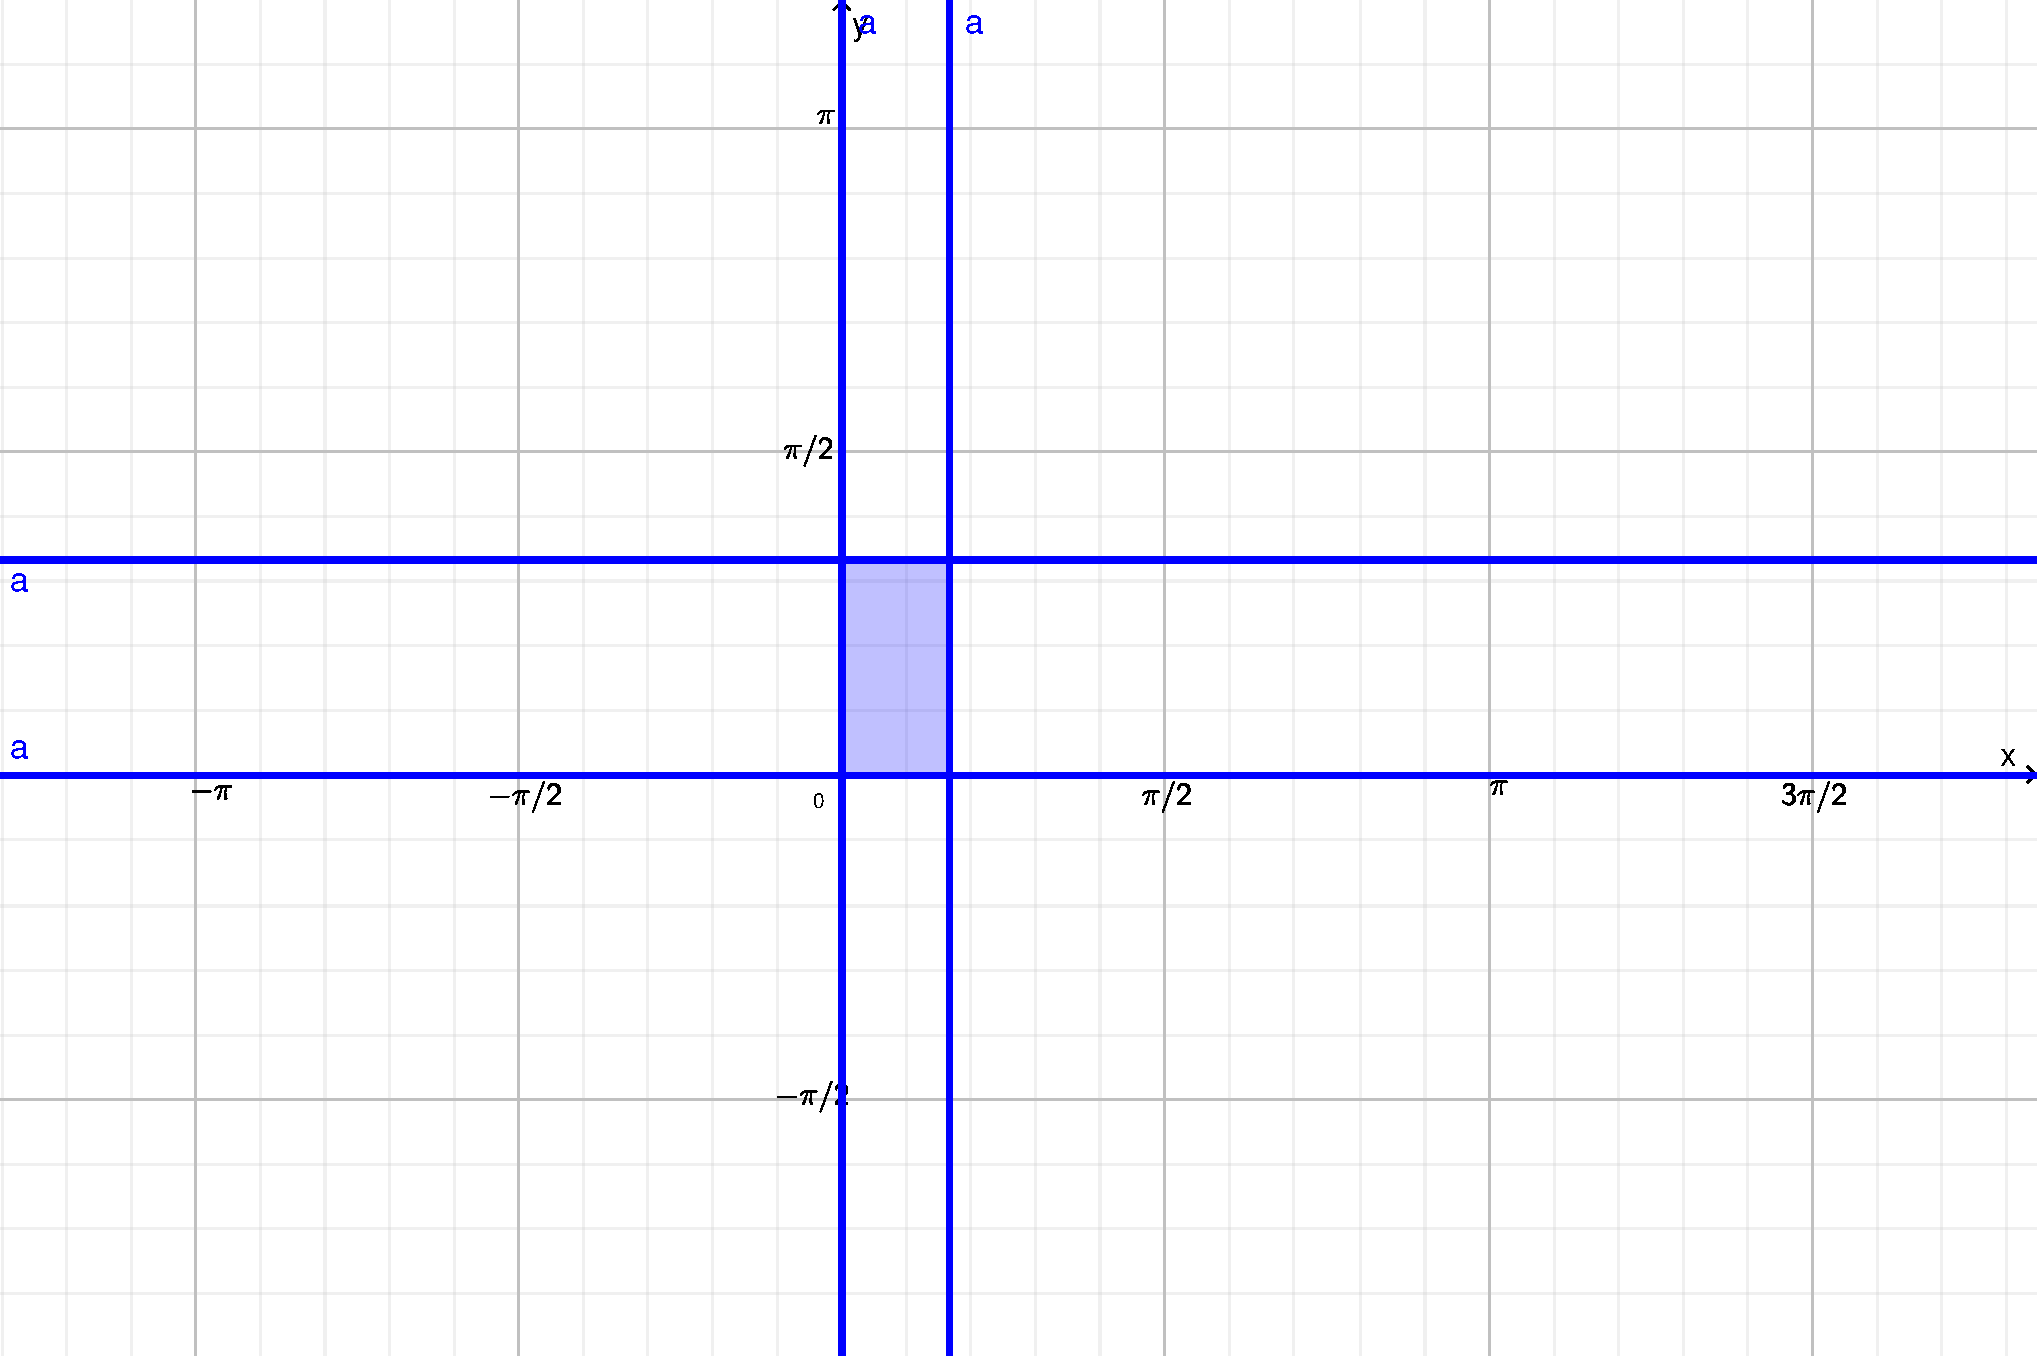
\includegraphics[width=0.7\linewidth]{fig/integrais-multiplas-1a}
		\caption{Região de integração}
		\label{fig:integrais-multiplas-1a}
	\end{figure}
	
	\begin{equation*}
		S = \int_{0}^{\frac{\pi}{6}} \int_{0}^{\frac{\pi}{3}} x \sen (x + y) dy dx
	\end{equation*}
	
	\begin{equation*}
		S = - \int_{0}^{\frac{\pi}{6}} \left[ x \cos (x + y) \right]_0^{\frac{\pi}{3}} dx
	\end{equation*}
	
	\begin{equation*}
		S = - \int_{0}^{\frac{\pi}{6}} \left[ x \cos \left(x + \frac{\pi}{3}\right) - \cos (x) \right] dx
	\end{equation*}
	
	\begin{equation*}
		S = \int_0^{\frac{\pi}{6}} \cos (x) dx - \int_0^{\frac{\pi}{6}} x \cos \left( x + \frac{\pi}{3}\right)
	\end{equation*}

	\begin{equation*}
		S = \left[ \sen (x) \right]_0^{\frac{\pi}{6}} -
		\left( \left[x \sen \left(x + \frac{\pi}{3}\right)\right]_0^{\frac{\pi}{6}} - \int_{0}^{\frac{\pi}{6}} \sen (x) dx \right)
	\end{equation*}
	
	\begin{equation*}
		S = \frac{1}{2} - 0 -
		\left( \left[ \frac{\pi}{6} \sen \left( \frac{\pi}{6} + \frac{\pi}{3} \right) - 0 \right] - \left[ \cos (x) \right]_0^{\frac{\pi}{6}} \right)
	\end{equation*}
	
	\begin{equation*}
		S = \frac{1}{2} - \left( \left[ \frac{\pi}{6} \sen \left( \frac{\pi}{2} \right) - 0 \right] - \left[ \cos \left(\frac{\pi}{6}\right) - \cos \left( 0 \right) \right] \right)
	\end{equation*}
	
	\begin{equation*}
		S = \frac{1}{2} - \left( \frac{\pi}{6} - \left[ \frac{\sqrt{3}}{2} - 1 \right] \right)
	\end{equation*}
	
	\begin{equation*}
		S = \frac{3}{6} - \frac{\pi}{6} + \frac{3\sqrt{3}}{6} - \frac{6}{6} \right]
	\end{equation*}
	
	\begin{equation*}
		S = \frac{-3-\pi+3\sqrt{3}}{6}
	\end{equation*}
	
	\begin{equation*}
		S = \frac{3\sqrt{3}-3-\pi}{6}
	\end{equation*}
	
	
	\section*{Questão 2}
	
	Dada a integral tripla $ \int_{0}^{2} \int_{0}^{\frac{y}{2}} \int_{0}^{y-2x} dz dx dy $, desenvolva os seguintes itens.
	
	\begin{enumerate}[a]
		\item Faça a descrição analítica do domínio de integração.
		\item Faça a descrição gráfica da região de integração no plano xy.
		\item Calcule a integral dada. O que o resultado pode significar?
		\item Qual a função que delimita o sólido inferiormente e qual a função que delimita o sólido superiormente?
	\end{enumerate}
	
	(Valor da questão: 1,0)
	
	\section*{Questão 3}
	
	Dada a integral $ \int \int_R x \exp{xy} dA $, sendo que R é a região dos pontos do plano xy dada pelo produto cartesiano $ R=[0, 1] \times [0, 1] $.
	
	\begin{enumerate}[a]
		\item Fazer a descrição analítica da região de integração.
		\item Fazer a descrição gráfica da região de integração.
		\item Escrever a integral em diferentes ordens de integração
		\item Calcular a integral usando a ordem mais conveniente.
	\end{enumerate}

	(Valor da questão: 1,0)
	
	\section*{Questão 4}
	
	Determinar o volume do sólido delimitado por:
	
	$ z = 2x+3y+4 $
	
	$ x = 0 $
	
	$ x = 1 $
	
	$ y = 0 $
	
	$ y = 2 $
	
	(Valor da Questão: 1.0)
	
	\section*{Questão 5}
	
	Calcule a integral dupla $ \int \int_R \exp{\frac{y}{x}} dA $, sendo R a região dada por:
	
	$ y = x^3 $
	
	$ y = x $
	
	$ 1 \le x \le 2 $
	
	O cálculo obtido representa a área da região R? Justifique a sua resposta
	
	(Valor da questão: 1,0)
	
	
	\section*{Questão 6}
	
	Usando integrais triplas, calcule o volume do sólido acima da superfície $ z = x^2 + y^2 $ e abaixo da superfície $ z = 4 - x^2 - y^2 $.
	
	(Valor da questão: 1,0)
	
	\section*{Questão 7}
	
	Calcule a seguinte integral usando coordenadas esféricas:
	
	$ \int \int \int_R (x^2 + y^2 + z^2)^2 dV $, sendo que B é a bola com sentro na origem e raio 4.
	
	\section*{Questão 8}
	
	Calcule $ \int_{0}^3 \int_{0}^{\sqrt{9-y^2}} \int_{\sqrt{x^2+y^2}}^{\sqrt{18-x^2-y^2}} (x^2 + y^2 + z^2) dz dx dy $. Use coordenadas esféricas. O resultado obtido representa um volume? Justifique a sua resposta.
	
	(Valor da questão: 1,0)
	
	
	\section*{Questão 9}
	
	Escolha algumas funções e tente fazer a modelagem de um sólido usando um software livre a sua esoclha. O sólido não deve ter o volume encontrado por fórmulas da Geometria. Relate aqui nessa questão essa sua experiência e apresente as funções escolindas e o sólido montado no software. Caso você pesquise em livros ou na internet, apresente aqui a referência bibliográfica.
	
	(Valor da questão: 1,0)
	
	\section*{Questão 10}
	
	Relate aqui sua participação nos Fóruns 1 e 2.
	S
\end{document}